\documentclass[%
pdf,
%nocolorBG,
colorBG,
slideColor,
%slideBW,
%draft,
%frames
%azure
%contemporain
%nuancegris
%troispoints
%lignesbleues
%darkblue
%alienglow
%autumn
]{prosper}
\usepackage{pifont, amsmath, multicol}
%\usepackage{floatflt, wrapfig,subfigure}
%\usepackage{wrapfig}
%\usepackage{floatflt}
\usepackage{color}
\usepackage{epsfig}
\usepackage{pifont}
\usepackage[T1]{fontenc}
\usepackage[latin1]{inputenc}
\def\QuotS#1#2{\leavevmode\kern-.0em\raise.2ex\hbox{$#1$}\kern-.1em/\kern-.1em\lower.25ex\hbox{$#2$}}


%\usepackage[francais]{babel}
%\def«{\og\ignorespaces}%
%\def»{{\fg}}%
\newcommand{\spacer}{\rule[-3mm]{0mm}{8mm}}

\newcommand{\RR}{\ensuremath{\mathbb{R}}}
\newcommand{\NN}{\ensuremath{\mathbb{N}}}
\newcommand{\QQ}{\ensuremath{\mathbb{Q}}}
\newcommand{\CC}{\ensuremath{\mathbb{C}}}
\newcommand{\ZZ}{\ensuremath{\mathbb{Z}}}
\newcommand{\TT}{\ensuremath{\mathbb{T}}}

\def\QuotS#1#2{\leavevmode\kern-.0em\raise.2ex\hbox{$#1$}\kern-.1em/\kern-.1em\lower.25ex\hbox{$#2$}}


\title{\Huge \textcolor{blue}{Zigzags in plane graphs}\\[3mm]
\textcolor{blue}{and generalizations}}

\author{
\textcolor{red}{\Large Michel Deza}\\[2mm]
\textcolor{red}{\large ENS/CNRS, Paris and ISM, Tokyo}\\[2mm]
\textcolor{red}{and}\\[2mm]
\textcolor{red}{\Large Mathieu Dutour}\\[2mm]
\textcolor{red}{\large ENS/CNRS, Paris and Hebrew University, Jerusalem}\\[2mm]
}
\author{
\textcolor{red}{\Large Mathieu Dutour}\\[2mm]
\textcolor{red}{\large ENS/CNRS, Paris and Hebrew University, Jerusalem}\\[2mm]
\textcolor{red}{and}\\[2mm]
\textcolor{red}{\Large Michel Deza}\\[2mm]
\textcolor{red}{\large ENS/CNRS, Paris and ISM, Tokyo}\\[2mm]
}


\slideCaption{}

\date{}



\begin{document}
\maketitle




\begin{slide}{}
\begin{center}
{\Huge 
\begin{tabular*}{5cm}{c}
\\[-0.5cm]
\textcolor{blue}{I. }\textcolor{red}{Simple}\\
\textcolor{red}{two-faced}\\
\textcolor{red}{polyhedra}
\end{tabular*}
}
\end{center}
\end{slide}




\begin{slide}{Polyhedra and planar graphs}
A graph is called \textcolor{red}{$k$-connected} if after removing any set of $k-1$ vertices it remains connected.

\vspace{2mm}

The \textcolor{red}{skeleton} of a polytope $P$ is the graph $G(P)$ formed by its vertices, with two vertices adjacent if they generate a face of $P$.

\vspace{3mm}

{\em {\bf Theorem} (Steinitz)

(i) A graph $G$ is the skeleton of a $3$-polytope if and only if it is planar and $3$-connected.

(ii) $P$ and $P'$ are in the same \textcolor{red}{combinatorial type} if and only if $G(P)$ is isomorphic to $G(P')$.
}

\vspace{3mm}

The \textcolor{red}{dual} graph $G^*$ of a plane graph $G$ is the plane graph formed by the faces of $G$, with two faces adjacent if they share an edge.


\end{slide}



\begin{slide}{Simple two-faced polyhedra}
A polyhedron is called \textcolor{red}{simple} if all its vertices are $3$-valent.
If one denote $p_i$ the number of faces of \textcolor{red}{gonality} $i$, then Euler's relation take the form:
\begin{equation*}
12=\sum_{i} (6-i) p_i\;.
\end{equation*}
A simple planar graph is called \textcolor{red}{two-faced} if the gonality of its faces has only two possible values:
\begin{center}
$a$ and $b$, where $3\leq a< b\leq 6$.
\end{center}

\vspace{3mm}

We consider mainly classes $q_n$, i.e. simple planar graphs with $n$ vertices and $(a,b)=(q,6)$; 
\begin{center}
there are $3$ cases: $3_n$, $4_n$, $5_n$.
\end{center}


\end{slide}


\begin{slide}{}
{\tiny
\begin{tabular}{||c||c|c|c|c||}
\hline
\hline
$(a,b)$ & Polyhedra & Exist if and only if & $p_a$ & $n$\\ \hline\hline
$(5,6)$ & $5_{n}$ (\textcolor{red}{fullerenes}) & $p_6\in N-\{1\}$& $p_5=12$ &$n=20+2p_6$\\ \hline
$(4,6)$ & $4_{n}$ & $p_{6} \in N-\{1\}$ & $p_4=6$ &$n=8+2p_6$\\ \hline
$(3,6)$ & $3_{n}$ & $p_{6}/2 \in N-\{1\}$ & $p_3=4$ &$4+2p_6$\\  \hline\hline
$(4,5)$ & 4 dual deltahedra & $p_5=2,3,4,5$ &$p_4=5,4,3,2$&$n=10,12,14,16$\\ \hline
$(3,5)$ & D\"urer's Octahedron & $p_5=6$ &$p_3=2$ &$n=12$\\ \hline
$(3,4)$ & Prism${}_{3}$ & $p_4=3$ & $p_3=2$ & $n=6$\\ 
\hline
\hline
\end{tabular}
}
\begin{center}
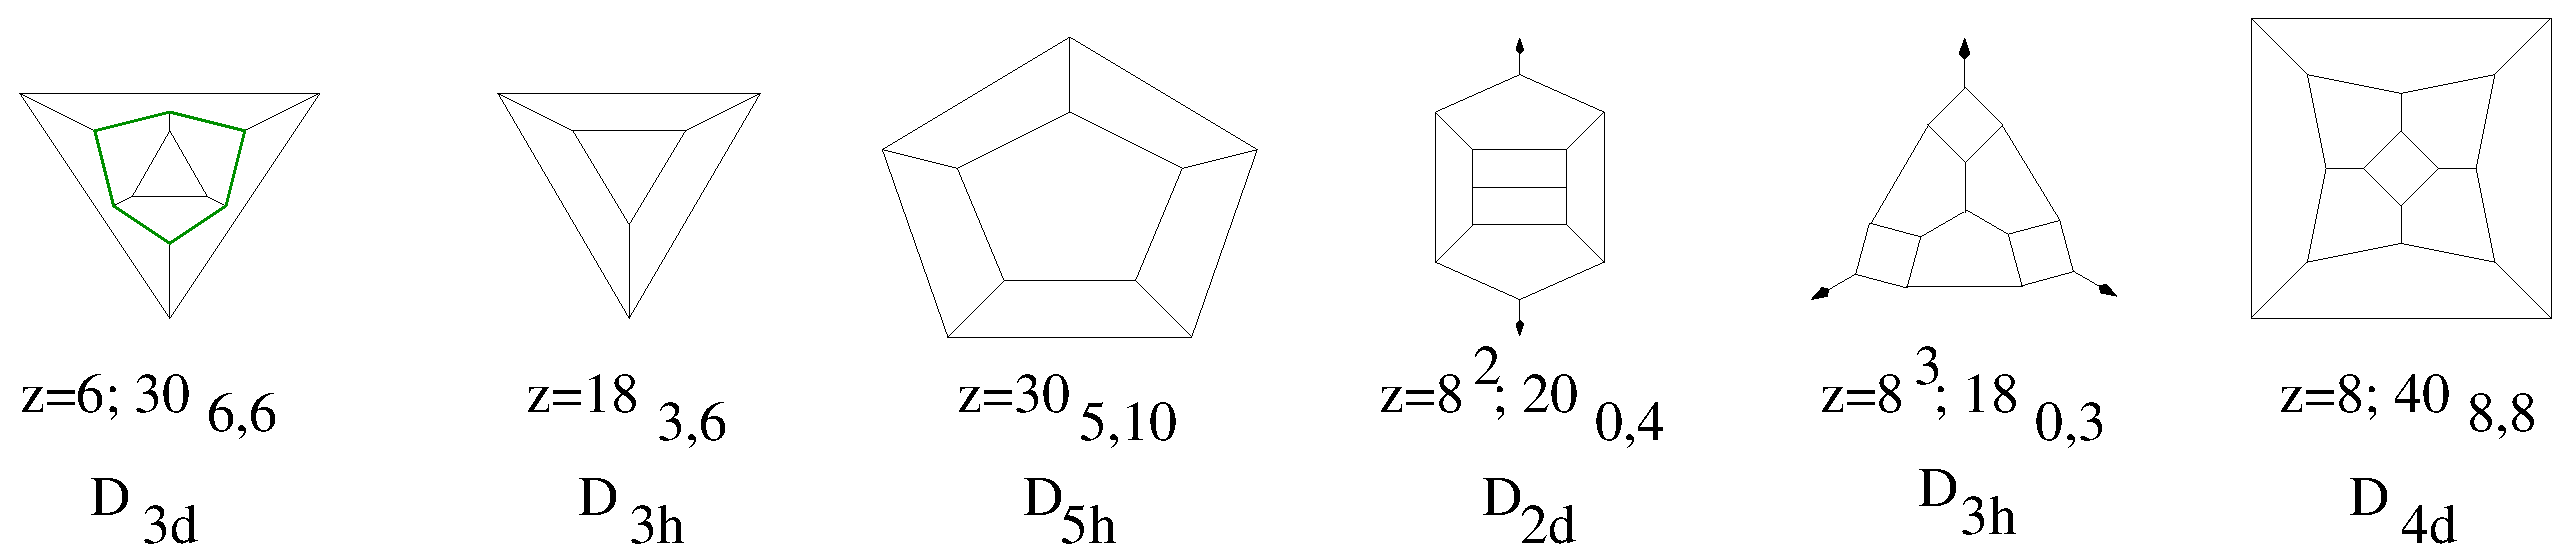
\epsfig{file=ZIGZAGpicture/Deltahedra-orga2.eps, width=11cm}
\end{center}

\vspace{-3mm}

\end{slide}



\overlays{3}{
\begin{slide}{$k$-connectedness}
\fromSlide{1}{
{\em {\bf Theorem}

\begin{enumerate}
\item[(i)] Any 3-valent plane graph without (>6)-gonal faces is $2$-connected.

\vspace{2mm}

\item[(ii)] Moreover, any 3-valent plane graph without (>6)-gonal faces is $3$-connected except of the following serie $G_n$:

\end{enumerate}
}}
\onlySlide*{1}{\begin{center}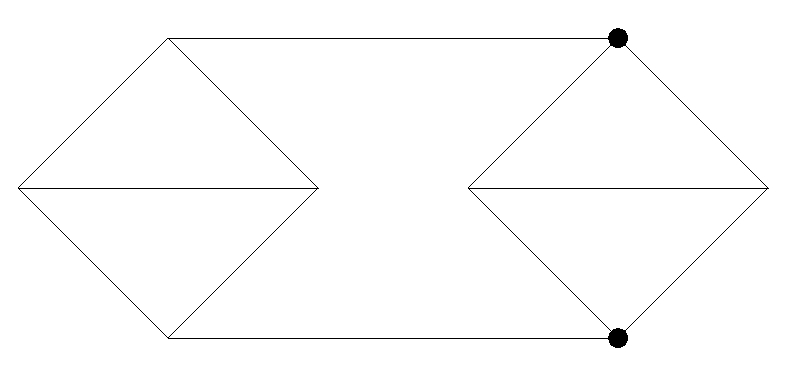
\epsfig{file=ZIGZAGpicture/2connected1.eps,width=6cm}\end{center}}%
\onlySlide*{2}{\begin{center}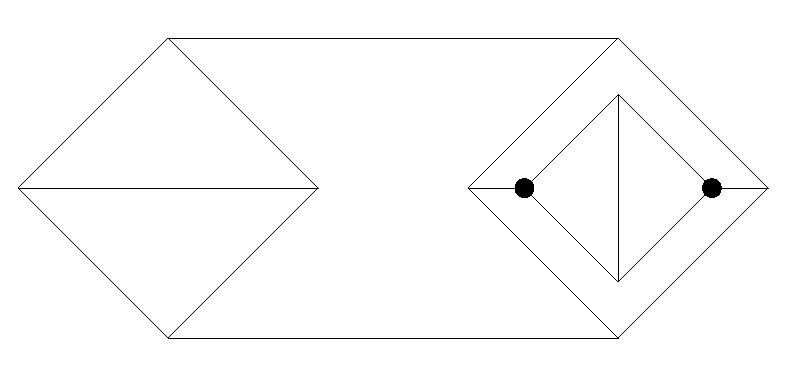
\epsfig{file=ZIGZAGpicture/2connected2.eps,width=6cm}\end{center}}%
\onlySlide*{3}{\begin{center}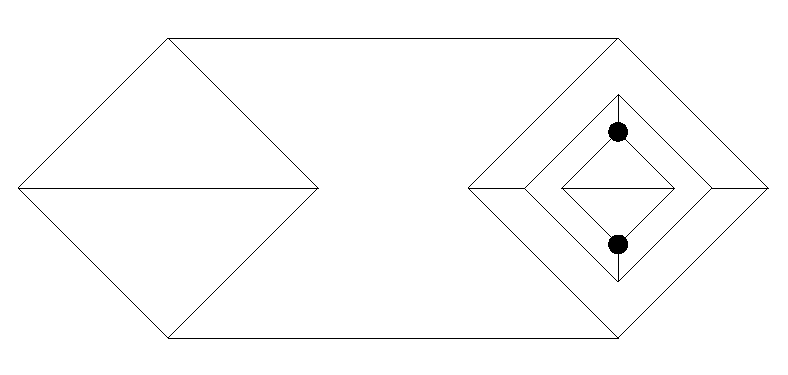
\epsfig{file=ZIGZAGpicture/2connected3.eps,width=6cm}\end{center}}%


\end{slide}
}
%\begin{center}
%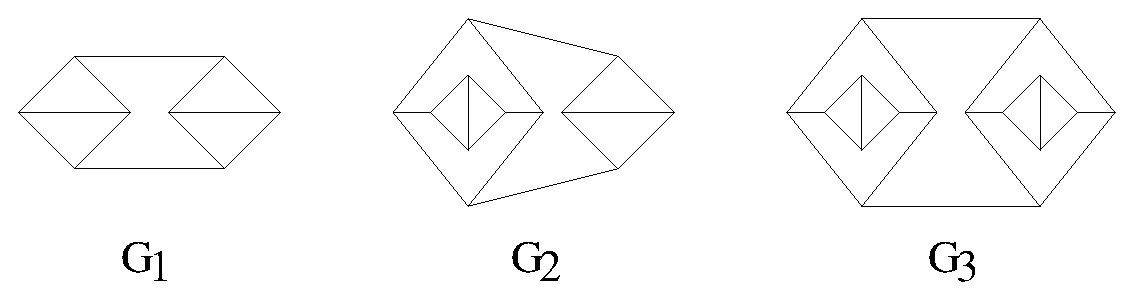
\epsfig{file=SequenceGraph.eps,width=10cm}
%\end{center}



\begin{slide}{Point groups}
(point group) $Isom(P)\subset Aut(G(P))$ (combinatorial group)

{\em {\bf Theorem}(Mani, 1971)

Given a $3$-connected planar graph $G$, there exist a $3$-polytope $P$, whose group of isometries is isomorphic to $Aut(G)$ and $G(P)=G$.
}

\vspace{3mm}

So, $Aut(G)$ of plane graphs $G$ are finite subgroups of $O(3)$.

The symmetry groups of graphs $q_n$ are known:

\begin{enumerate}
\item[\ding{108}] For \textcolor{red}{$3_n$}: $D_{2}$, $D_{2h}$, $D_{2d}$, $T$, $T_d$ (Fowler and al.)

\item[\ding{108}] For \textcolor{red}{$4_n$}: $C_1$, $C_s$, $C_2$, $C_{i}$, $C_{2v}$, $C_{2h}$, $D_2$, $D_3$, $D_{2d}$, $D_{2h}$, $D_{3d}$, $D_{3h}$, $D_6$, $D_{6h}$, $O$, $O_h$ (Dutour and Deza)
\item[\ding{108}] For \textcolor{red}{$5_n$}: $C_1$, $C_2$, $C_i$, $C_s$, $C_3$, $D_2$, $S_4$, $C_{2v}$, $C_{2h}$, $D_3$, $S_6$, $C_{3v}$, $C_{3h}$, $D_{2h}$, $D_{2d}$, $D_5$, $D_6$, $D_{3h}$, $D_{3d}$, $T$, $D_{5h}$, $D_{5d}$, $D_{6h}$, $D_{6d}$, $T_d$, $T_h$, $I$, $I_h$ (Fowler and al.)
\end{enumerate}

\end{slide}



\begin{slide}{}
\begin{center}
{\Huge 
\begin{tabular*}{5cm}{c}
\\[0.5cm]
\textcolor{blue}{II. }\textcolor{red}{Zigzags}
\end{tabular*}
}
\end{center}
\end{slide}

%%%%%%%%%%%%%%   Zig Zags
\overlays{6}{
\begin{slide}{Zigzags}
\onlySlide*{1}{\begin{center}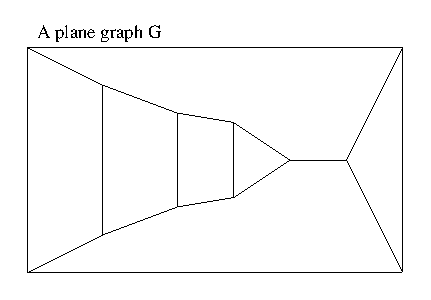
\epsfig{file=ZIGZAGpicture/ZigZagSample1.eps,width=11cm}\end{center}}%
\onlySlide*{2}{\begin{center}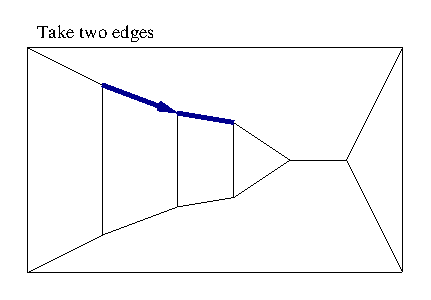
\epsfig{file=ZIGZAGpicture/ZigZagSample2.eps,width=11cm}\end{center}}%
\onlySlide*{3}{\begin{center}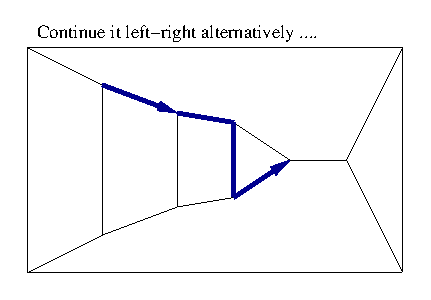
\epsfig{file=ZIGZAGpicture/ZigZagSample3.eps,width=11cm}\end{center}}%
\onlySlide*{4}{\begin{center}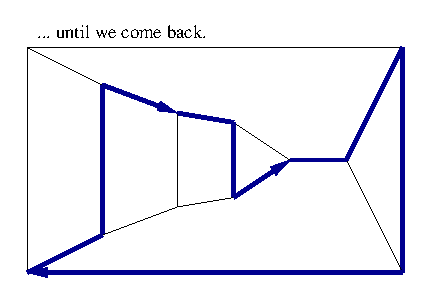
\epsfig{file=ZIGZAGpicture/ZigZagSample4.eps,width=11cm}\end{center}}%
\onlySlide*{5}{\begin{center}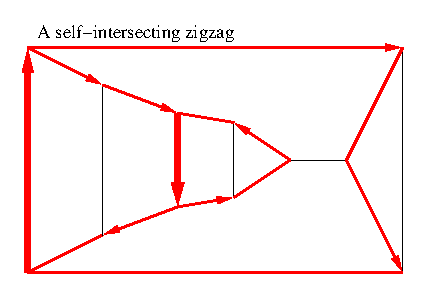
\epsfig{file=ZIGZAGpicture/ZigZagSample5.eps,width=11cm}\end{center}}%
\onlySlide*{6}{\begin{center}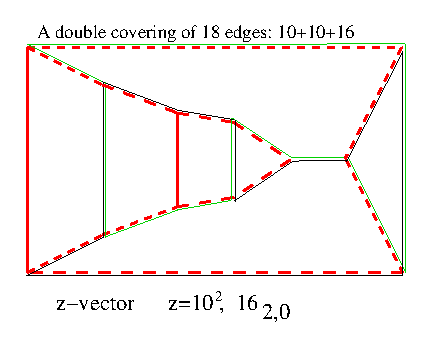
\epsfig{file=ZIGZAGpicture/ZigZagSample6.eps,width=9.8cm}\end{center}}%
\end{slide}
}


\overlays{2}{
\begin{slide}{Intersection Types}
\fromSlide{1}{
\vspace{-2mm}
Let $Z$ and $Z'$ be (possibly, $Z=Z'$) zigzags of a plane
graph $G$ and let an orientation be selected on them. An edge of
intersection $Z\cap Z'$ is called of \textcolor{red}{type I} or \textcolor{red}{type II}, if $Z$ and $Z'$ traverse $e$ in opposite or same direction, respectively
%
%\vspace{2mm}

\begin{center}
\epsfxsize=90mm
\epsfbox{ZIGZAGpicture/TypeI_TypeII-pres.eps}
\end{center}
%
%\vspace{2mm}
}%
\fromSlide{2}{
The types of self-intersection depends on orientation chosen on zigzags except if $Z=Z'$:

\begin{center}
\epsfxsize=80mm
\epsfbox{ZIGZAGpicture/TypeI_TypeIIsec.eps}
\end{center}

}%

\end{slide}
}


\begin{slide}{Zigzag parameters}

\begin{enumerate}
\item[\ding{108}] The \textcolor{red}{signature} of a zigzag $Z$ is
the pair $(\alpha_1,\alpha_2)$, where $\alpha_1$ and $\alpha_2$ are the
numbers of its edges of self-intersection of type I and type II, respectively.

\vspace{1mm}

\item[\ding{108}] The \textcolor{red}{intersection vector $Int(Z)$} lists
pairs of intersection $(\alpha_1, \alpha_2)$ with all other zigzags.

\vspace{1mm}

\item[\ding{108}] \textcolor{red}{z-vector} of $G$ is the
vector enumerating \textcolor{red}{lengths} (numbers of edges) of all its
zigzags with their signature as subscript.



\end{enumerate}

\begin{center}
\begin{minipage}{3cm}
\epsfxsize=25mm
\epsfbox{ZIGZAGpicture/Graph12_6sec.eps}
\end{minipage}
\begin{minipage}{7cm}
$2$ zigzags with $Int=(1,3), (3,3)$\\
$1$ self-intersecting with $Int=(3,3)^{2}$
\end{minipage}
\end{center}

\end{slide}







\begin{slide}{Duality and types}

{\em {\bf Theorem}

The zigzags of a plane graph $G$ are in one-to-one correspondence with zigzags of $G^*$.
The length is preserved, but intersection of type I and II are interchanged.

}

\vspace{2mm}

{\em {\bf Theorem}

Let $G$ be a plane graph; for any orientation of all zigzags of $G$, we have:

(i) The number of edges of type II, which are incident to any fixed \textcolor{red}{vertex}, is even.

(ii) The number of edges of type I, which are incident to any fixed \textcolor{red}{face}, is even.
}


\end{slide}





\begin{slide}{Bipartite graphs}

{\em {\bf Remark}
A plane graph is \textcolor{red}{bipartite} if and only if its faces have even gonality.
}



{\em {\bf Theorem} (Shank-Shtogrin)

For any planar bipartite graph $G$ there exist an orientation of zigzags, with respect to which each edge has type I.
}


\begin{center}
\begin{minipage}{5.5cm}
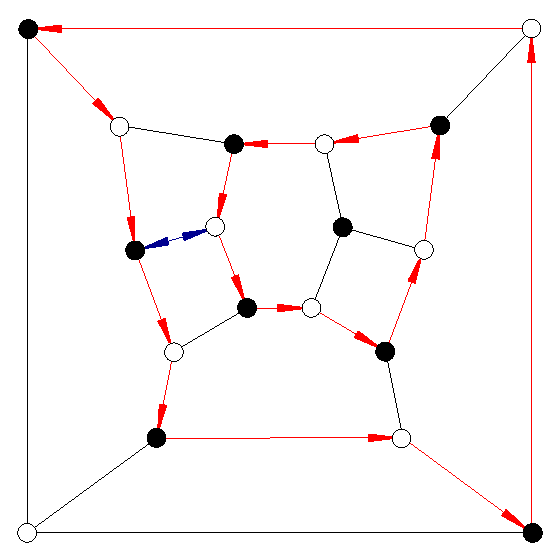
\epsfig{file=ZIGZAGpicture/ExampleBipartitionSec2.eps, width=5cm}
\end{minipage}
\begin{minipage}{3cm}
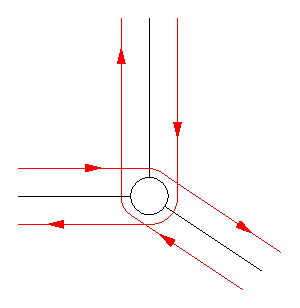
\epsfig{file=ZIGZAGpicture/LocalDraw.eps, width=3cm}
\end{minipage}
\end{center}





\end{slide}


\begin{slide}{Zigzag properties of a graph}
{\scriptsize
\begin{enumerate}
\item[\ding{108}] \textcolor{red}{$z$-uniform}: all zigzags have the same length and signature, 
\item[\ding{108}] \textcolor{red}{$z$-transitive}: symmetry group is transitive on zigzags,
\item[\ding{108}] \textcolor{red}{$z$-knotted}: there is only one zigzag,
\item[\ding{108}] \textcolor{red}{$z$-balanced}: all zigzags of the same length and signature, have identical intersection vectors.
\end{enumerate}
}
All known $z$-uniform $3$-valent graphs are $z$-balanced.

\begin{center}
\begin{minipage}[b]{3.7cm}
\centering
\epsfig{figure=ZIG2picture/FirstUnbalancedTrig.eps,height=2cm}\par
{\tiny $18$-vertices $(C_2)$, $z=8^3; 30_{2,5}$}
\end{minipage}
\begin{minipage}[b]{3.7cm}
\centering
\epsfig{figure=ZIG2picture/FirstUnbalanced4n.eps,height=2cm}\par
{\tiny $4_{72}$($C_1$), $z=30_{1,0}, 54^2_{4,0}, 78_{13, 0}$}
\end{minipage}
\begin{minipage}[b]{3.7cm}
\centering
\epsfig{figure=ZIG2picture/FirstUnbalanced5n.eps,height=2cm}\par
{\tiny $5_{52}$($D_{2d}$),\par
 $z=16^4; 92_{12, 12}$}
\end{minipage}
\end{center}
\vspace{-2mm}
\begin{center}
{\tiny Smallest (among all $3$-valent, all $4_n$, all $5_n$) $z$-unbalanced $3$-valent graphs}
\end{center}

\end{slide}







\begin{slide}{Zigzags of reg. and semireg. polyhedra}

\begin{center}
{\scriptsize
\begin{tabular}{||c|c|c|c||}
\hline
\hline
\#\,edges&polyhedron& $z$-vector&int. vector \\ \hline
\hline
6  &\textcolor{red}{Tetrahedron}&$4^3$&$(1,1)^2$\\ 
12 &\textcolor{red}{Cube, Octahedron}&$6^4$&$(0,2)^3$\\ 
%12 &\textcolor{red}{Octahedron}&$6^4$&$2^3$\\ 
30 &\textcolor{red}{Dodecahedron, Icosahedron}&$10^6$&$(0,2)^5$\\\hline
%30 &\textcolor{red}{Icosahedron}&$10^6$&$2^5$\\ \hline
24 &\textcolor{red}{Cuboctahedron}&$8^6$&$(0,2)^4,(0,0)$ \\%=Med(cube)=Med(octahedron)
60 &\textcolor{red}{Icosidodecahedron}&$10^{12}$&$(0,2)^5,(0,0)^6$ \\%=Med(ico.)=Med(dode.)
48 &\textcolor{red}{Rhombicuboctahedron}&$12^8$&$(0,2)^6,(0,0)$\\ %=Med(cuboctahedron)
120&\textcolor{red}{Rhombicosidodecahedron}&$20^{12}$&$(0,2)^{10},(0,0)$\\ %=Med(icosidodecahedron)
72 &\textcolor{red}{Truncated Cuboctahedron}&$18^8$&$(0,6),(0,2)^6$\\ 
180&\textcolor{red}{Truncated Icosidodecahedron}&$30^{12}$&$(0,10),(0,2)^{10}$\\ 
18 &\textcolor{red}{Truncated Tetrahedron}&$12^3$&$(3,3)^2$\\ 
36 &\textcolor{red}{Truncated Octahedron}&$12^6$&$(0,4),(0,2)^4$\\ 
\hline
\hline
\end{tabular}
}
\end{center}
\end{slide}






\begin{slide}{}

\begin{center}
{\scriptsize
\begin{tabular}{||c|c|c|c||}
\hline
\hline
36 &\textcolor{red}{Truncated Cube}&$18^4$&$(2,4)^3$\\
90 &\textcolor{red}{Truncated Icosahedron}&$18^{10}$&$(0,2)^9$\\ 
90 &\textcolor{red}{Truncated Dodecahedron}&$30^6$&$(2,4)^5$\\ 
60 &\textcolor{red}{Snub Cube}&$30_{3,0}^4$&$(4,4)^3$\\ 
150&\textcolor{red}{Snub Dodecahedron}&$50_{5,0}^6$&$(4,4)^5$\\ \hline
3m &$Prism_m$, $m\equiv 0 \pmod{4}$&$(\frac{3m}{2})^4$&$(0,\frac{m}{2})^3$\\
3m &$Prism_m$, $m\equiv 2 \pmod{4}$&$({3m}_{\frac{m}{2},0})^2$&$(0,2m)$\\ 
3m &$Prism_m$, $m\equiv 1,3 \pmod{4}$&${6m}_{m,2m}$&\\ 
4m &$APrism_m, m \equiv 0 \pmod{3}$&$(2m)^4$&$(0,\frac{2m}{3})^3$\\ 
4m &$APrism_m, m \equiv 1,2 \pmod{3}$&$2m;6m_{0,2m}$&\\ \hline\hline
84 &\textcolor{red}{Klein map}(oriented, genus $3$ surface)&$8^{21}$&$(0,1)^8, {0}^{12}$\\
48 &\textcolor{red}{Dyck map}(oriented, genus $3$ surface)&$6^{16}$&$(0,1)^6, {0}^9$\\
\hline
\hline
\end{tabular}
}
\end{center}


\end{slide}







\begin{slide}{First generalizations of zigzags}
\vspace{3mm}

Above Table contains plane graphs, which are not $3$-valent, and non-planar graphs.

\vspace{6mm}

In fact, the notion of zigzag can be easily generalized on any \textcolor{blue}{plane graph} and on a graph, embedded in any \textcolor{blue}{oriented surface}.

\vspace{6mm}

Moreover, this notion, being local, can be generalized even for \textcolor{blue}{non-oriented surfaces}.


\end{slide}



\begin{slide}{Perfect matching on $5_n$ graphs}
\begin{center}
\begin{minipage}{57mm}
{\scriptsize
Let $G$ be a $z$-knotted graph $5_n$. 
\begin{enumerate}
\item[(i)] $z=n_{\alpha_1, \alpha_2}$ with $\alpha_1\geq \frac{n}{2}$. If $\alpha_1=\frac{n}{2}$ then the edges of type I form a perfect matching $PM$
\item[(iii)] every face incident to two or zero edges of $PM$
\item[(iv)] two faces, $F_1$ and $F_2$ are incident to zero edges of $PM$, $PM$ is organized around them in concentric circles.
\end{enumerate}
}
\end{minipage}
\begin{minipage}{5.5cm}
\epsfxsize=55mm
\epsfbox{ZIGZAGpicture/ZZkekule34sec.eps}
\end{minipage}



\end{center}

{\scriptsize

M. Deza, M. Dutour and P.W. Fowler, {\em Zigzags, Railroads and Knots in Fullerenes}, Journal of Chemical Information and Computer Sciences, {\bf 44-4} (2004) 1282-1293.
}

\end{slide}






%\begin{slide}{}
%\begin{center}
%{\Huge 
%\begin{tabular*}{10cm}{c}
%\\[-1.2cm]
%\textcolor{blue}{III. }\textcolor{red}{Four Tables}\\
%\textcolor{red}{on zigzags notions}\\
%\textcolor{red}{for fullerenes $5_n$}\\
%{\large \textcolor{red}{(from Deza, Dutour and Fowler)}}
%\end{tabular*}
%}
%\end{center}
%
%\end{slide}





%\begin{slide}{$z$-uniform $5_n$ with $n\leq 60$}
%\vspace{-7mm}
%\begin{center}
%{\tiny
%\begin{tabular}{|c||c|c|c|c|}
%\hline
%$\,\,n$&isomer    &orbit lengths& $z$-vector    &  int. vector\\
%\hline
%$20$& $I_h$:1     &$6$         &$10_{0,0}^6$   &  $2\sp{5}$\\
%$28$& $T_d$:2     &$4$,$3$     &$12_{0,0}^7$   &  $2\sp{6}$\\
%$40$& $T_d$:40    &$4$         &$30_{0,3}^4$   &  $8\sp{3}$\\
%$44$& $T$:73      &$3$         &$44_{0,4}^3$   &  $18\sp{2}$\\
%$44$& $D_2$:83    &$2$         &$66_{5,10}^2$  &  $36$\\
%$48$& $C_2$:84    &$2$         &$72_{7,9}^2$   &  $40$\\
%$48$& $D_3$:188   &$3$,$3$,$3$ &$16_{0,0}^9$   &  $2\sp{8}$\\
%$52$& $C_3$:237   &$3$         &$52_{2,4}^3$   &  $20\sp{2}$\\
%$52$& $T$:437     &$3$         &$52_{0,8}^3$   &  $18\sp{2}$\\
%$56$& $C_2$:293   &$2$         &$84_{7,13}^2$  &  $44$\\
%$56$& $C_2$:349   &$2$         &$84_{5,13}^2$  &  $48$\\
%$56$& $C_3$:393   &$3$         &$56_{3,5}^3$   &  $20\sp{2}$\\
%$60$& $C_2$:1193  &$2$         &$90_{7,13}^2$  &  $50$\\
%$60$& $D_2$:1197  &$2$         &$90_{13,8}^2$  &  $48$\\
%\textcolor{red}{$60$}& $D_3$:1803  &$6$,$3$,$1$ &\textcolor{red}{$18_{0,0}^{10}$}&  \textcolor{red}{$2\sp{9}$}\\
%\textcolor{blue}{$60$}& $I_h$:1812  &$10$        &\textcolor{blue}{$18_{0,0}^{10}$}&  \textcolor{blue}{$2\sp{9}$}\\
%\hline
%\end{tabular}
%}
%\end{center}

%\begin{center}
%All $z$-uniform $5_n$ with $n\leq 60$ (DDF)
%\end{center}
%
%\begin{enumerate}
%\item M. Deza, M. Dutour and P.W. Fowler, {\em Zigzags, Railroads and Knots in Fullerenes}, (2002).
%\end{enumerate}


%\end{slide}





%\begin{slide}{$z$-uniform \textcolor{red}{IPR} $5_n$ with $n\leq 100$}
%
%\begin{center}
%{\tiny
%\begin{tabular}{|c||c|c|c|c|}
%\hline
%$\,\,n$&isomer    &orbit lengths& $z$-vector    &  int. vector\\
%\hline
%$80$&$I_h$:7    &$12$   &$20_{0,0}^{12}$ &$0,2\sp{10}$\\
%\textcolor{red}{$84$}&$T_d$:20   &$6$    &\textcolor{red}{$42_{0,1}^{6}$}  &\textcolor{red}{$8\sp{5}$}\\
%\textcolor{blue}{$84$}&$D_{2d}$:23&$4$,$2$&\textcolor{blue}{$42_{0,1}^{6}$}  &\textcolor{blue}{$8\sp{5}$}\\
%$86$&$D_3$:19   &$3$    &$86_{1,10}^{3}$ &$32\sp{2}$\\
%$88$&$T$:34     &$12$   &$22_{0,0}^{12}$ &$2\sp{11}$\\
%$92$&$T$:86     &$6$    &$46_{0,3}^6$    &$8\sp{5}$\\
%$94$&$C_3$:110  &$3$    &$94_{2,13}^3$   &$32\sp{2}$\\
%$100$&$C_2$:387 &$2$    &$150_{13,22}^2$ &$80$\\
%$100$&$D_2$:438 &$2$    &$150_{15,20}^2$ &$80$\\
%\textcolor{red}{$100$}&\textcolor{red}{$D_2$}:432 &\textcolor{red}{$2$}    &\textcolor{red}{$150_{17,16}^2$} &\textcolor{red}{$84$}\\
%\textcolor{blue}{$100$}&\textcolor{blue}{$D_2$}:445 &\textcolor{blue}{$2$}    &\textcolor{blue}{$150_{17,16}^2$} &\textcolor{blue}{$84$}\\
%\hline
%\end{tabular}
%}
%\end{center}
%\textcolor{red}{IPR} means the absence of adjacent pentagonal faces;
%
%IPR enhanced stability of putative fullerene molecule.


%\begin{center}
%All $z$-uniform $5_n$ with $n\leq 60$ (DDF)
%\end{center}
%
%\begin{enumerate}
%\item M. Deza, M. Dutour and P.W. Fowler, {\em Zigzags, Railroads and Knots in Fullerenes}, (2002).
%\end{enumerate}
%\end{slide}







%\begin{slide}{IPR $z$-knotted $5_n$ with $n\leq 100$}
%\begin{center}
%\begin{minipage}{5.5cm}
%{\tiny
%\begin{tabular}{|c||c|c|}
%\hline
%$\,\,n$  &signature &isomers\\
%\hline
%86       &$43,86^{\textcolor{red}{*}}$&$C_2$:$2$\\
%90       &$47,88$&$C_1$:$7$\\
%         &$53,82$&$C_2$:$19$\\
%         &$71,64$&$C_2$:$6$\\
%94       &$47,94^{\textcolor{red}{*}}$&$C_1$:$60$; $C_2$:$26$, $126$\\
%         &$65,76$&$C_2$:$121$\\
%         &$69,72$&$C_2$:$7$\\
%96       &$49,95$&$C_1$:$65$\\
%         &$53,91$&$C_1$:$7$, $37$, $63$\\
%\hline
%\end{tabular}
%}
%\end{minipage}
%\begin{minipage}{5.5cm}
%{\tiny
%\begin{tabular}{|c||c|c|}
%\hline
%98       &$49,98^{\textcolor{red}{*}}$&$C_2$:$191$, $194$, $196$\\
%         &$63,84$&$C_1$:$49$\\
%         &$75,72$&$C_1$:$29$\\
%         &$77,70$&$C_1$:$5$; $C_2$:$221$\\
%100      &$51,99$&$C_1$:$371$, $377$; $C_3$:$221$\\
%         &$53,97$&$C_1$:$29$, $113$, $236$\\
%         &$55,95$&$C_1$:$165$\\
%         &$57,93$&$C_1$:$21$\\
%         &$61,89$&$C_1$:$225$\\
%         &$65,85$&$C_1$:$31$, $234$\\
%\hline
%\end{tabular}
%}
%\end{minipage}
%\end{center}
%The symbol \textcolor{red}{${}^*$} above means that fullerene forms a \textcolor{red}{K\'ekule structure}, i.e. edges of self-intersection of type I cover exactly once the vertex-set of the fullerene graph (in other words, they form a \textcolor{red}{perfect matching} of the graph).
%
%
%\end{slide}



%\begin{slide}{Statistics of $z$-knotted $5_n$ with $n\leq 74$}
%\begin{center}
%\begin{minipage}{4.5cm}
%{\tiny
%\begin{tabular}{|c||c|c|}
%\hline
%$\,\,n$  &\# of $5_n$&\# of $z$-knotted\\
%\hline
%$34$&    $6$&$1$\\
%$36$&   $15$&$0$\\
%$38$&   $17$&$4$\\
%$40$&   $40$&$1$\\
%$42$&   $45$&$6$\\
%$44$&   $89$&$9$\\
%$46$&  $116$&$15$\\
%$48$&  $199$&$23$\\
%$50$&  $271$&$30$\\
%$52$&  $437$&$42$\\
%\hline
%\end{tabular}
%}
%\end{minipage}
%\begin{minipage}{3.5cm}
%{\tiny
%\begin{tabular}{|c||c|c|}
%\hline
%$54$&  $580$&$93$\\
%$56$&  $924$&$87$\\
%$58$& $1205$&$186$\\
%$60$& $1812$&$206$\\
%$62$& $2385$&$341$\\
%$64$& $3465$&$437$\\
%$66$& $4478$&$567$\\
%$68$& $6332$&$894$\\
%$70$& $8149$&$1048$\\
%$72$&$11190$&$1613$\\
%$74$&$14246$&$1970$\\
%\hline
%\end{tabular}
%}
%\end{minipage}
%\end{center}
%It will be interesting to estimate the relative order of magnitude of $z$-knotted fullerenes among all $5_n$ and of $z$-knotted $3$-valent graphs among all of them.
%
%\end{slide}





\begin{slide}{}
\begin{center}
{\Huge 
\begin{tabular*}{6cm}{c}
\\[-0.5cm]
\textcolor{blue}{III. }\textcolor{red}{Railroad}\\
\textcolor{red}{structure of}\\
\textcolor{red}{graphs $q_n$}
\end{tabular*}
}
\end{center}
\end{slide}

\begin{slide}{Railroads}

A \textcolor{red}{railroad} in graph $q_n$, $q=3, 4, 5$ is a circuit of hexagonal faces, such that any of them is adjacent to its neighbors on opposite faces. Any railroad is bordered by two zigzags.

\begin{center}
\begin{minipage}{5.5cm}
\centering
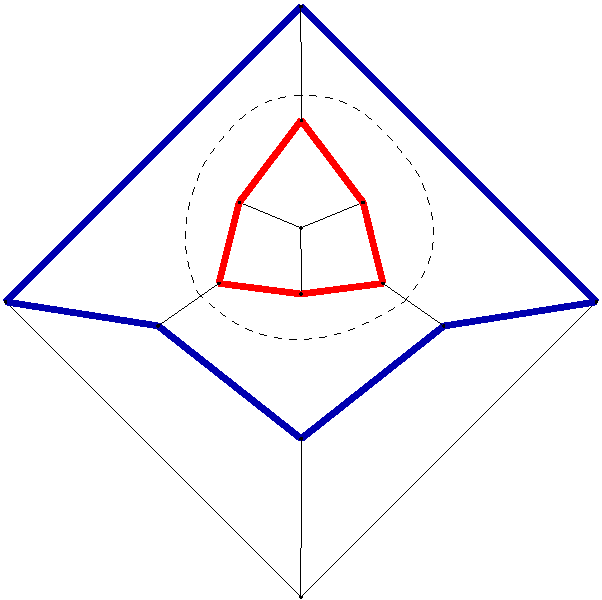
\epsfig{file=ZIGZAGpicture/Graph4n_14_1sec, height=4cm}\par
$4_{14}(D_{3h})$
\end{minipage}
\begin{minipage}{5.5cm}
\centering
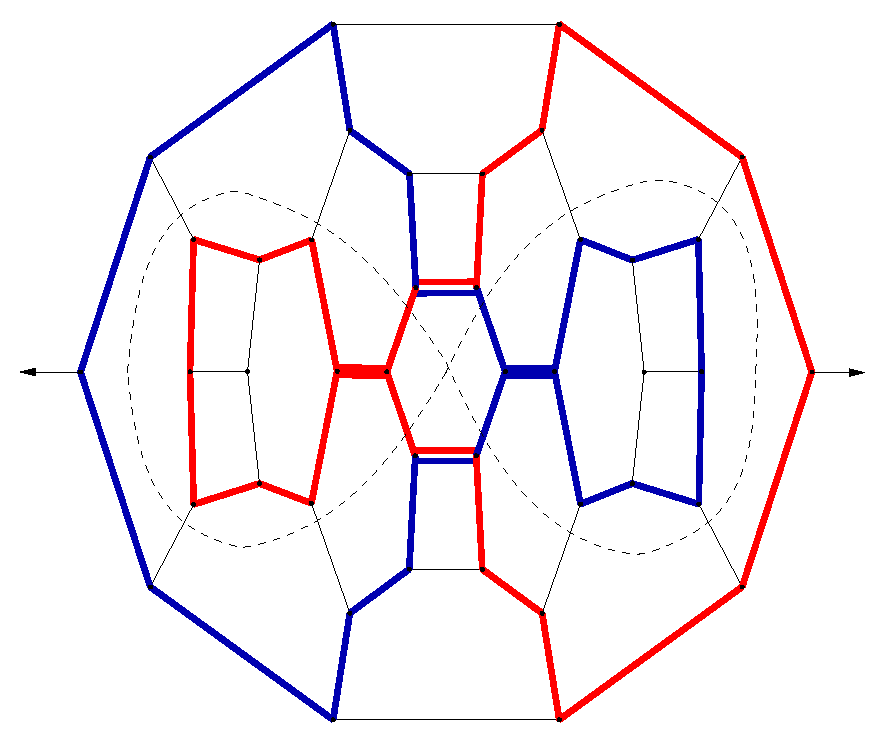
\epsfig{file=ZIGZAGpicture/Graph42_54th.eps, height=4cm}\par
$4_{42}(C_{2v})$
\end{minipage}
\end{center}

Railroads, as well as zigzags, can be self-intersecting (\textcolor{red}{doubly} or \textcolor{red}{triply}). A graph is called \textcolor{red}{tight} if it has no railroad.



\end{slide}


\begin{slide}{$4_{66}(D_{3h})$ with \textcolor{red}{triply} self-int. railroad}

\vspace{-2mm}
\begin{center}
\centering
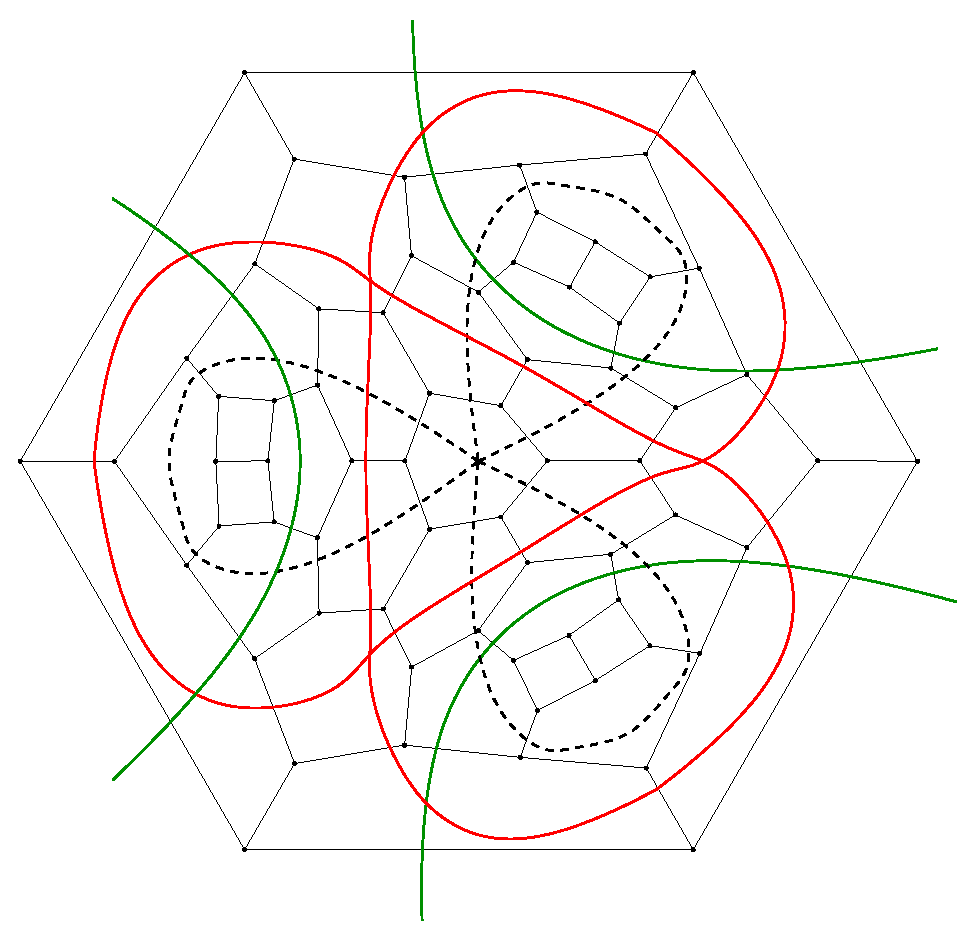
\epsfig{file=ZIGZAGpicture/ZZint111Railroad066_11-color.eps, height=7cm}\par
It is smallest such $4_n$. \textcolor{green}{Green} railroad also triply self-int.
\end{center}




\end{slide}






\begin{slide}{Railroads with triple points in small $4_n$}

\vspace{-2mm}
\begin{center}
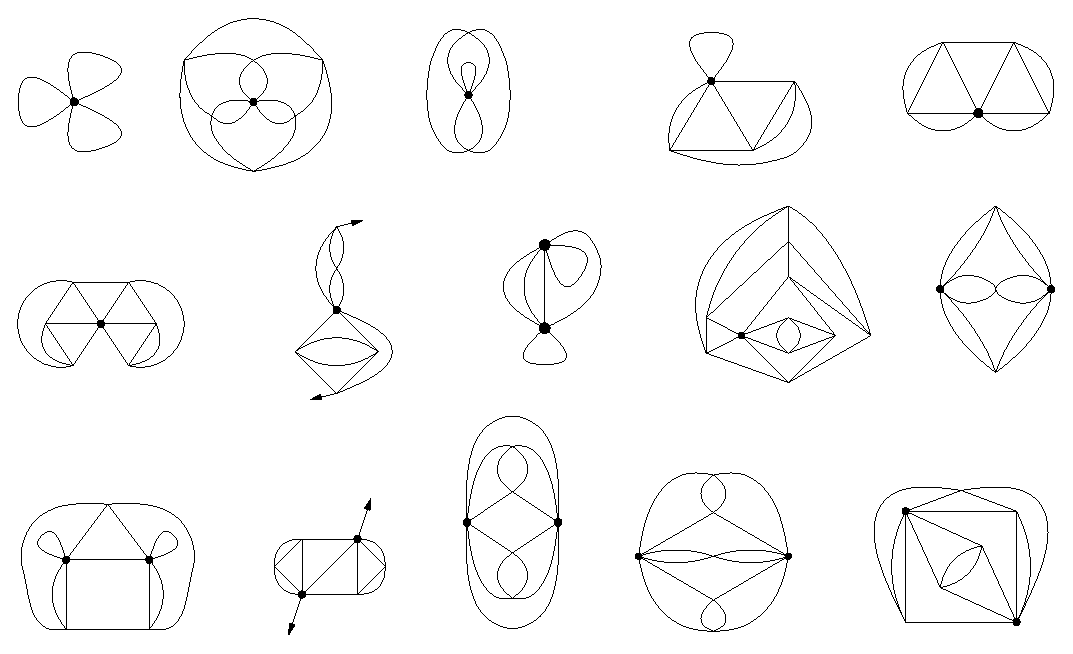
\epsfig{file=ZIGZAGpicture/CurveByTripleRailroad-orga2.eps, height=7cm}
\end{center}

\end{slide}




\begin{slide}{Railroads and pseudo-roads of $4_{126}(D_{3h})$}

\begin{center}
\begin{minipage}[b]{5.7cm}%
\centering
\epsfig{figure=ZIGZAGpicture/RailRoadSystemCurveSelf-color.eps,height=4.5cm}\par
{\scriptsize One of two self-intersecting railroads and the equatorial simple railroad}
\end{minipage}
\begin{minipage}[b]{5.5cm}%
\centering
\epsfig{figure=ZIGZAGpicture/RailRoadSystemPseudo-color.eps,height=5cm}\par
{\scriptsize All twelve pseudo-roads}
\end{minipage}
\end{center}
A \textcolor{red}{pseudo-road} between $4$-gons $b$ and $c$ is a sequence of
hexagons $a_1$, \dots, $a_l$,
s.t. if $a_0=b$ and $a_{l+1}=c$, then any $a_i$,
$1\leq i\leq l$, is adjacent to $a_{i-1}$ and $a_{i+1}$ on
opposite edges.


\end{slide}


\begin{slide}{Triply intersecting railroad in $5_{172}(C_{3v})$}
\begin{center}
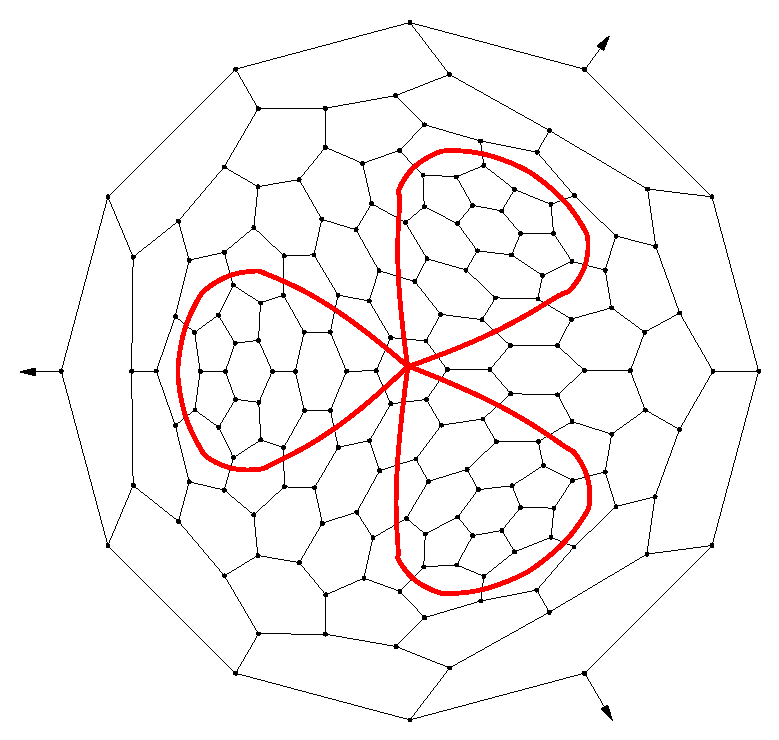
\epsfig{file=ZIGZAGpicture/DutourFull4th-color.eps,width=6cm}
\end{center}

\vspace{3mm}

{\em {\bf Conjecture: }
a railroad-curve of any $4_n$ appears in some $5_m$.
}


\end{slide}








\begin{slide}{Tight $5_n$ with only simple zigzags}
{\scriptsize
\begin{center}
\begin{tabular}{||c|c|l|c|c||}
\hline
\hline
$n$       &group          &$z$-vector     &orbit lengths  &int. vector\\
\hline \hline
$20$    &$I_h$          &$10^6$         &6              &$2^5$ \\
$28$    &$T_d$          &$12^7$         &3,4            &$2^6$\\
$48$    &$D_3$          &$16^9$         &3,3,3          &$2^8$\\
$60$    &$I_h$          &$18^{10}$      &10             &$2^9$\\
$60$    &$D_3$          &$18^{10}$      &1,3,6          &$2^9$\\
$76$    &$D_{2d}$       &$22^4,20^7$    &1,2,4,4        &$4,2^9$ and $2^{10}$\\
$88$    &$T$            &$22^{12}$      &12             &$2^{11}$\\
$92$    &$T_h$          &$22^6, 24^6$   &6,6            &$2^{11}$ and $2^{10}, 4$\\
$140$   &$I$            &$28^{15}$      &15             &$2^{14}$\\
\hline
\hline
\end{tabular}
\end{center}
}
Conjecture: this list is complete (checked for $n\leq 200$).

It gives $7$ \textcolor{red}{Gr\"unbaum arrangements} of plane curves.

\end{slide}




\begin{slide}{First IPR $5_n$ with self-intersect. railroad}
\begin{center}
\centering
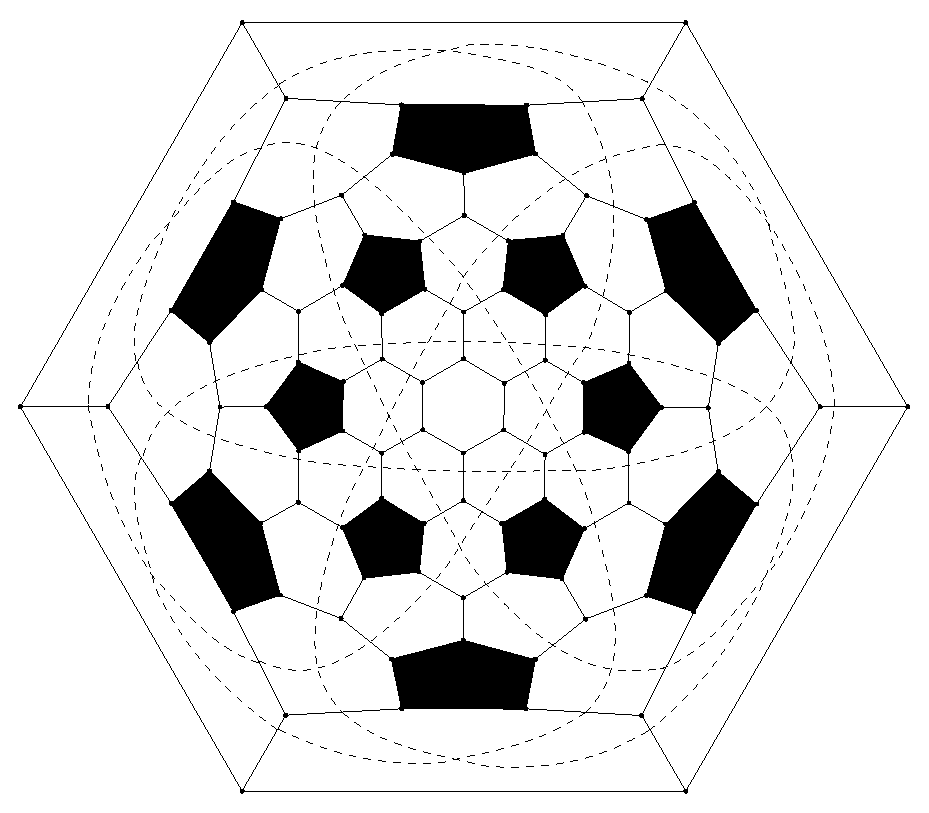
\epsfig{file=ZIGZAGpicture/DoorDraw.eps, height=75mm}\par
\end{center}
\end{slide}

\begin{slide}{IPR $5_{120}(C_{2v})$}
\begin{center}
\centering
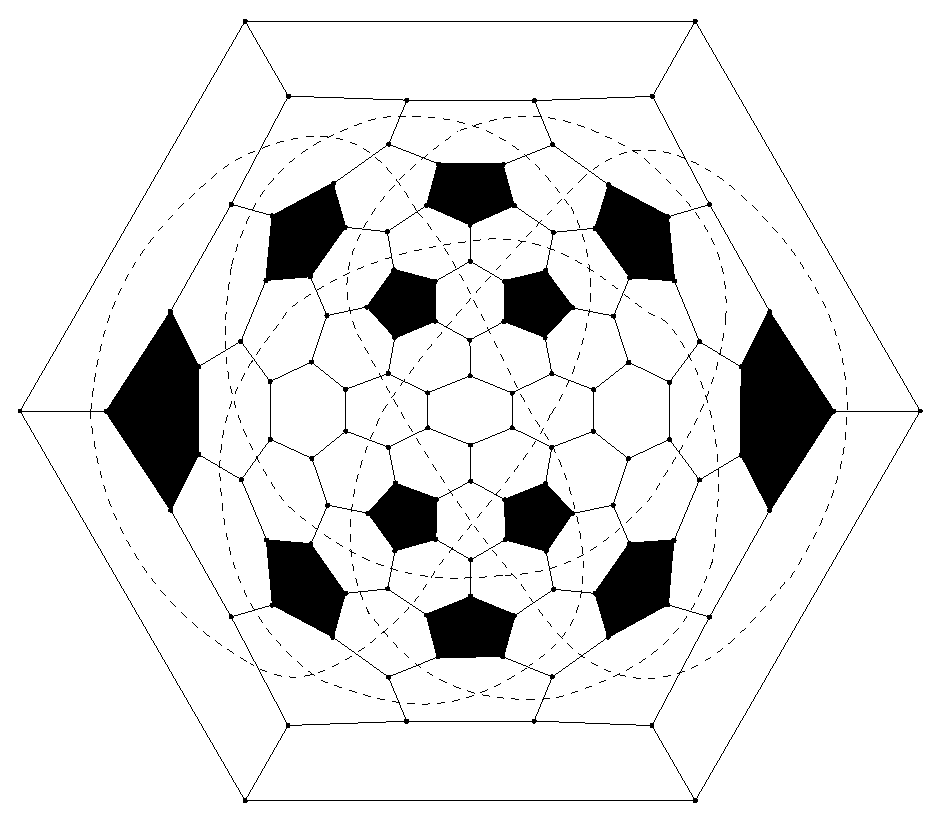
\epsfig{file=ZIGZAGpicture/ZZIPRselfRailroad120_10768_4th.eps, height=75mm}\par
\end{center}
\end{slide}

\begin{slide}{IPR $5_{120}(C_{2v})$}
\begin{center}
\centering
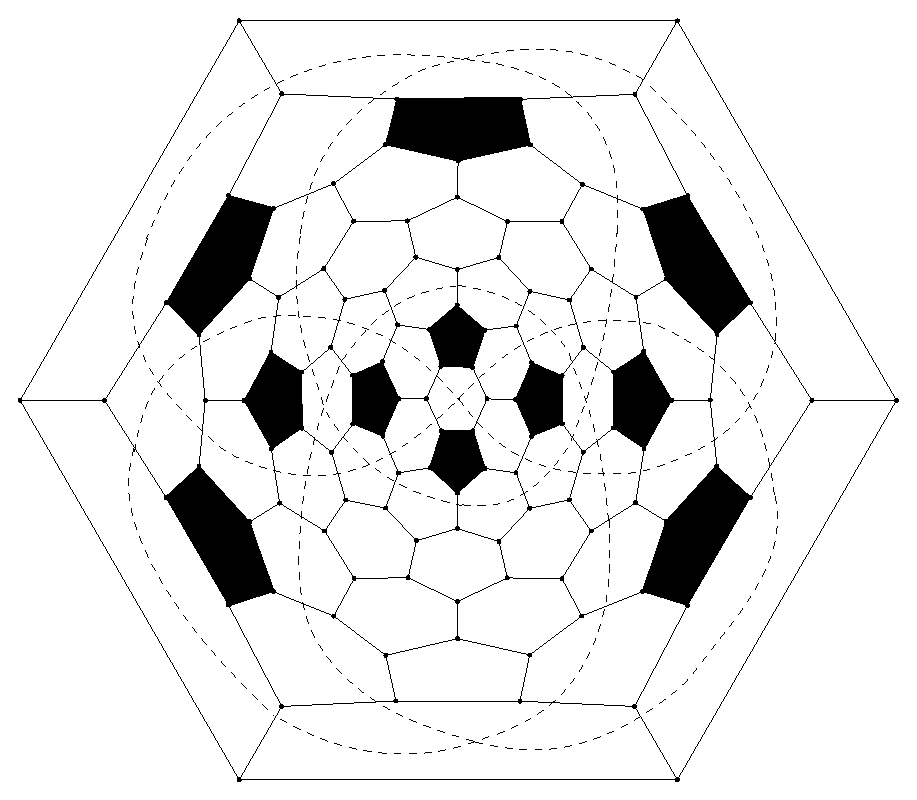
\epsfig{file=ZIGZAGpicture/ZZIPRselfRailroad120_10773_4th.eps, height=75mm}\par
\end{center}
\end{slide}

\begin{slide}{IPR $5_{120}(D_{5h})$}
\begin{center}
\centering
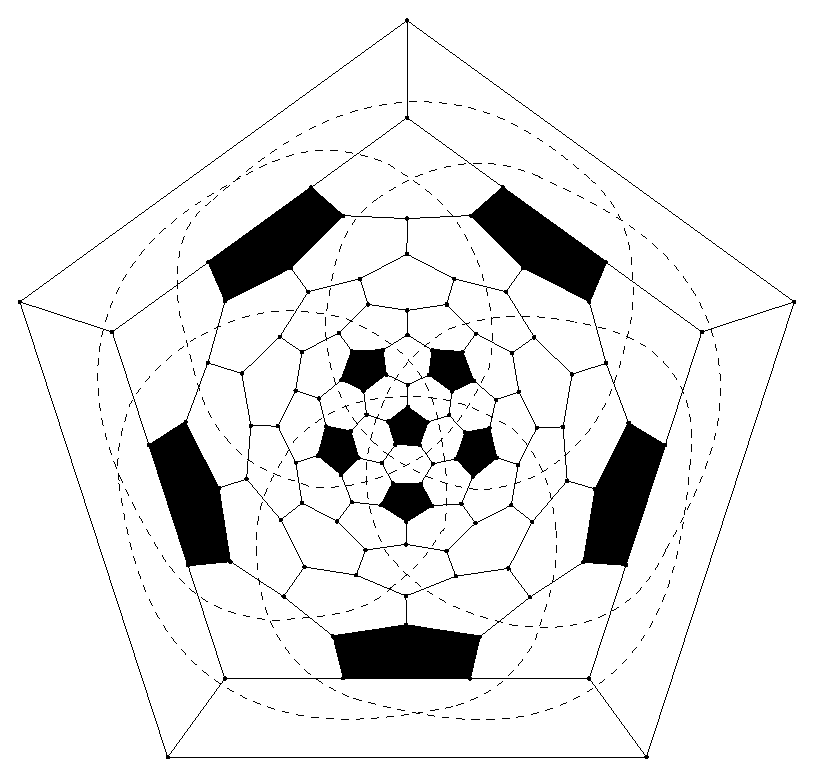
\epsfig{file=ZIGZAGpicture/ZZIPRselfRailroad120_10766_5th.eps, height=75mm}\par
\end{center}
\end{slide}












%\begin{slide}{Hexagon-triangle adjacencies for $3_n$}
%\vspace{-2mm}
%\begin{enumerate}
%\item[\ding{108}] no hexagon is adjacent to $\leq 2$ triangles; two cases:
%\begin{center}
%\begin{minipage}{3.5cm}
%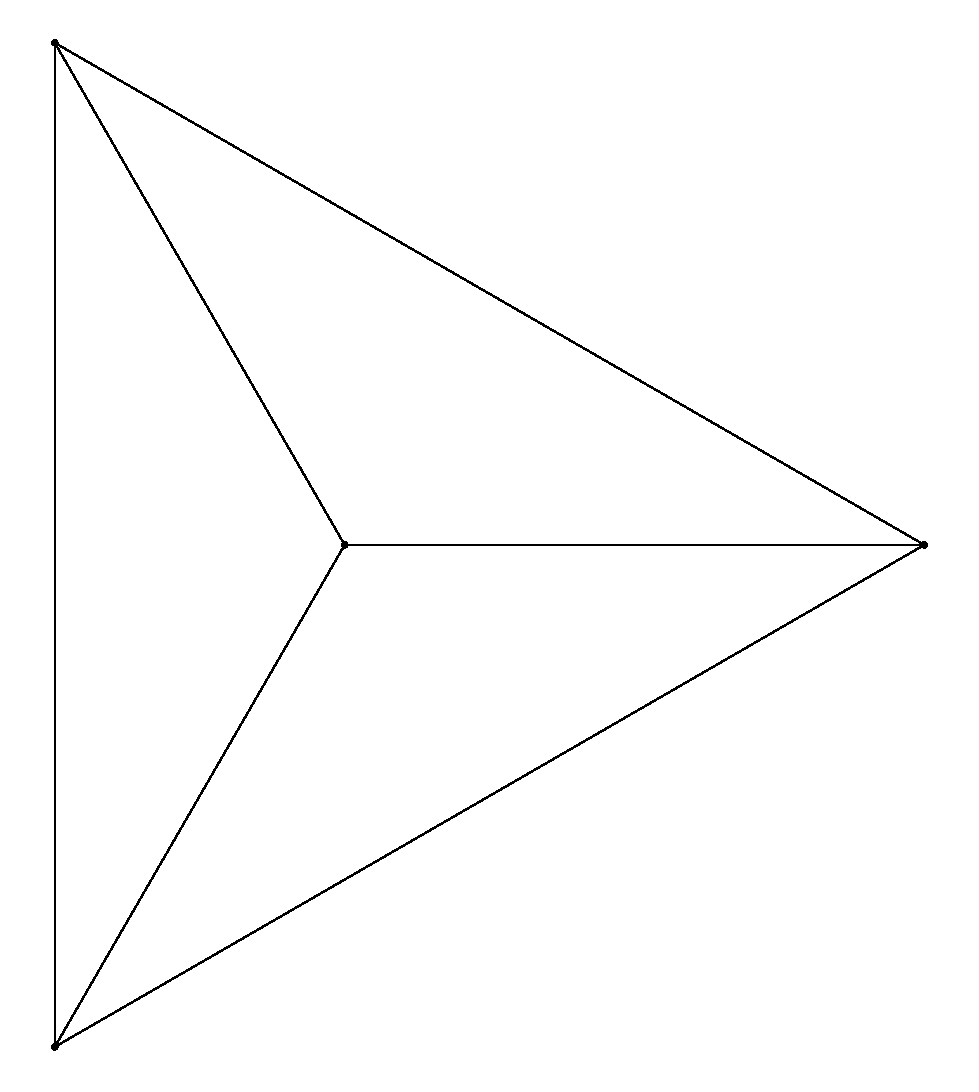
\epsfig{file=Tetrahedron.ps, height=1.5cm}
%\end{minipage}
%\begin{minipage}{3.5cm}
%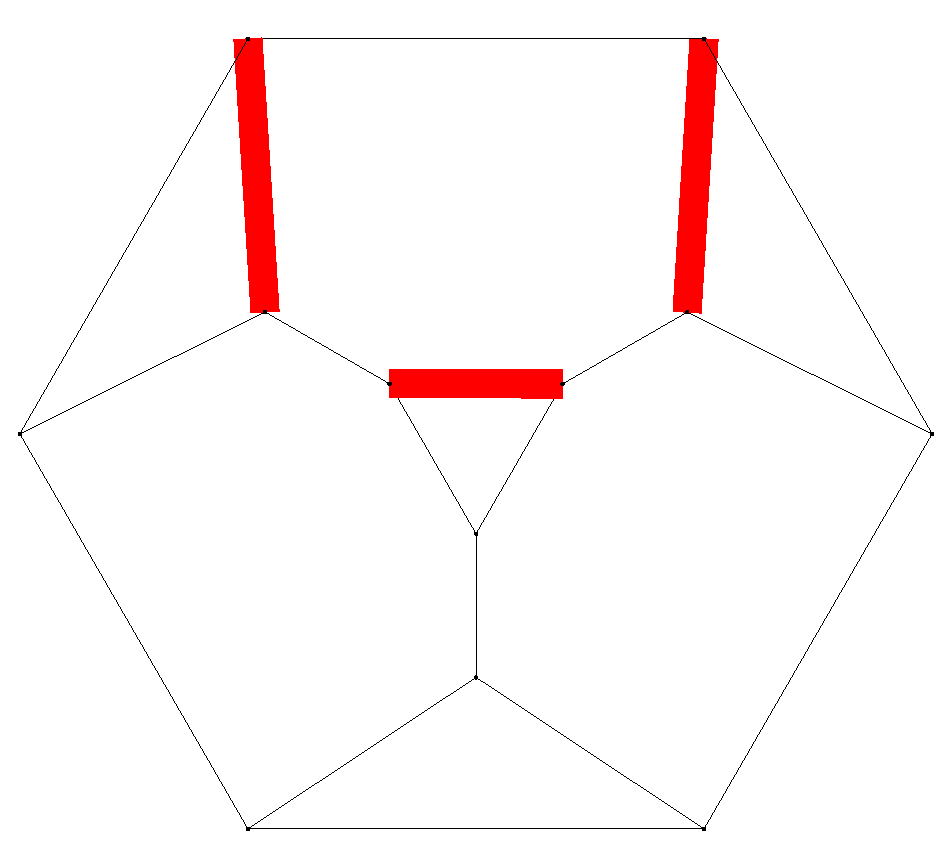
\epsfig{file=TruncatedTetrahedronSec.eps, height=1.5cm}
%\end{minipage}
%\end{center}
%\item[\ding{108}] any hexagon is adjacent to $0$ or $2$ triangles; two series
%\begin{center}
%\begin{minipage}[b]{2.5cm}%
%\centering
%\epsfig{figure=Graphiii24sec.eps,height=1.7cm}
%\end{minipage}
%\begin{minipage}[b]{2.5cm}%
%\centering
%\epsfig{figure=Graphiii28sec.eps,height=1.7cm}
%;
%\end{minipage}
%\begin{minipage}[b]{2.5cm}%
%\centering
%\epsfig{figure=First3nD2.sec.eps,height=1.7cm}
%\end{minipage}
%\begin{minipage}[b]{2.5cm}%
%\centering
%\epsfig{figure=Bigam32_2sec.eps,height=1.7cm}
%\end{minipage}
%\end{center}
%%some hexagons are adjacent to $1$ triangle
%\item[\ding{108}] others give a $5_n$ by collapsing of triangles
%\begin{center}
%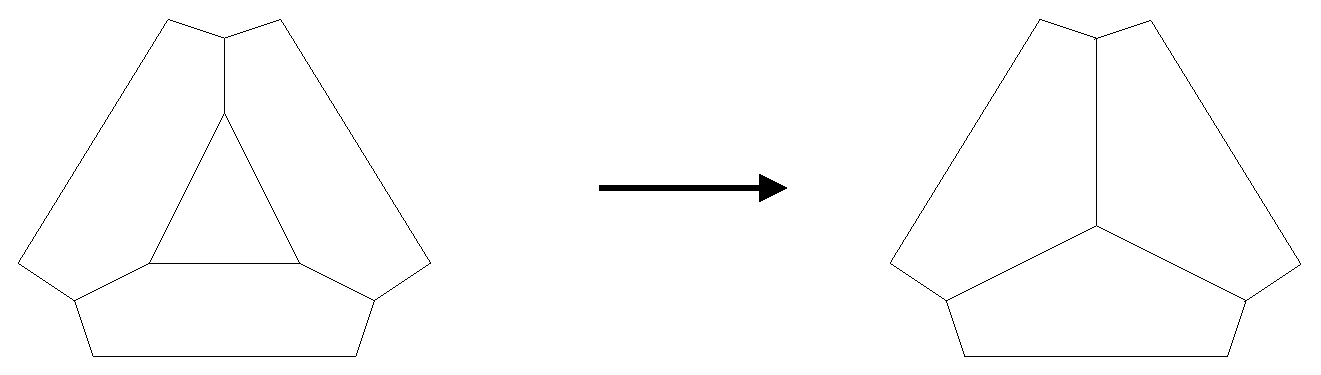
\epsfig{file=FowlerConstruction.eps, height=1.3cm}
%\end{center}
%
%\end{enumerate}
%
%\end{slide}




\begin{slide}{Comparing graphs $q_n$}

\vspace{-4mm}
\begin{center}
{\scriptsize 
\begin{tabular}{|c||c|c|c|}
\hline
q                            &$3$        &$4$                &$5$\\
\hline
\hline
max \# of zigzags in tight   &$3$       &$8(?)$               &$15(?)$\\
\hline
all tight with simple zigzags   &all tight  &Cube, Tr. Oct.     &$9$ examples(?)\\
\hline
int. size of $2$ simple zigzags &any even   &$2$, $4$, $6$      &any even\\
\hline
\end{tabular}
}
\begin{center}
\epsfig{figure=ZIGZAGpicture/ConstructionH8thisec-color.eps,height=5cm}
\end{center}

\end{center}


\end{slide}














\begin{slide}{}
\begin{center}
{\Huge 
\begin{tabular*}{6cm}{c}
\\[0.5cm]
\textcolor{blue}{IV. }\textcolor{red}{Parametrizing}\\
\textcolor{red}{graphs $q_n$}
\end{tabular*}
}
\end{center}
\end{slide}






\begin{slide}{Parametrizing graphs $q_n$}
\textcolor{red}{Idea}: the hexagons are of zero curvature, it suffices to give relative positions of faces of non-zero curvature.
\begin{itemize}
\item \textcolor{red}{Goldberg (1937)} All $3_n$, $4_n$ or $5_n$ of symmetry ($T$, $T_d$), ($O$, $O_h$) or ($I$, $I_h$) are given by Goldberg-Coxeter construction $GC_{k,l}$.
\item \textcolor{red}{Fowler and al. (1988)} All $5_n$ of symmetry $D_5$, $D_6$ or $T$ are described in terms of $4$ parameters.
\item \textcolor{red}{Graver (1999)} All $5_n$ can be encoded by $20$ integer parameters.
\item \textcolor{red}{Thurston (1998)} The $5_n$ are parametrized by $10$ complex parameters.
\item \textcolor{red}{Sah (1994)} Thurston's result implies that the Nrs of $3_n$, $4_n$, $5_n$ $\sim$ $n$, $n^3$, $n^9$.
\end{itemize}




\end{slide}





\begin{slide}{Goldberg-Coxeter construction}
Given a $3$-valent plane graph $G$, the zigzags of the Goldberg-Coxeter construction of $GC_{k,l}(G)$ are obtained by:

\begin{itemize}
\item Associating to $G$ two elements $L$ and $R$ of a group called \textcolor{red}{moving group},
\item computing the value of the \textcolor{red}{$(k,l)$-product} $L\odot_{k,l} R$,
\item the lengths of zigzags are obtained by computing the cycles structure of $L\odot_{k,l} R$.
\end{itemize}
For tight $5_n$ of symmetry $I$ or $I_h$ this gives $6$, $10$ or $15$ zigzags.


{\scriptsize

M. Dutour and M. Deza, {\em Goldberg-Coxeter construction for $3$- or $4$-valent plane graphs}, Electronic Journal of Combinatorics, {\bf 11-1} (2004) R20.
}


\end{slide}


\begin{slide}{The structure of graphs $3_n$}

\vspace{-4mm}
\begin{center}
\begin{minipage}{5cm}
\centering
\resizebox{5cm}{!}{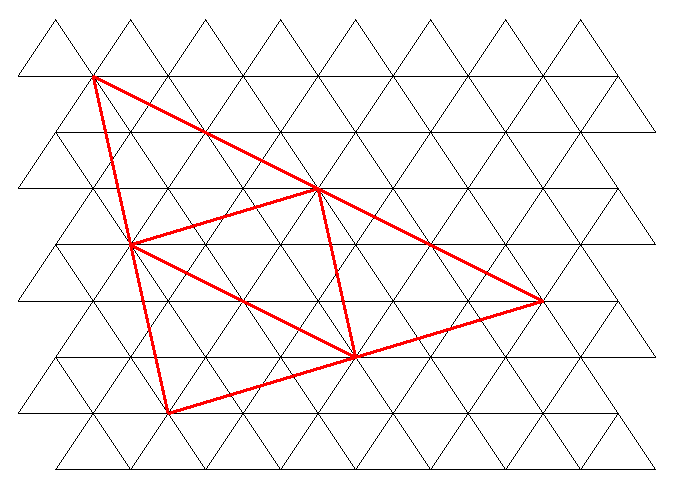
\includegraphics[bb=30 20 260 200, clip]{GOLDBERGpicture/Encoding3n.eps}}\par
$4$ triangles in $Z[\omega]$
\end{minipage}
\begin{minipage}{5cm}
\centering
\resizebox{5cm}{!}{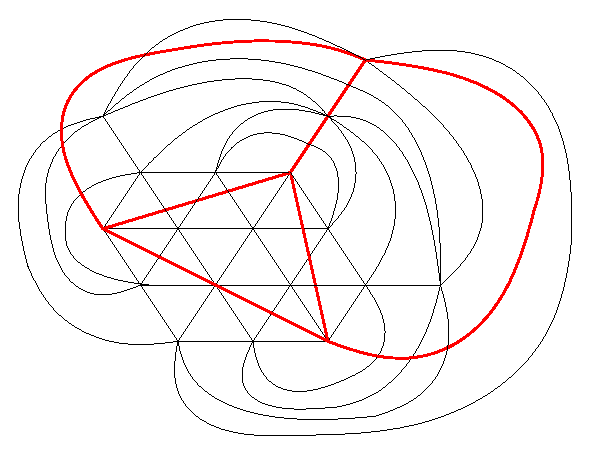
\includegraphics{GOLDBERGpicture/CorrespondingGraph3n.eps}}\par
The corresponding\par
triangulation
\end{minipage}
\end{center}

\begin{center}
\begin{minipage}{5cm}
\resizebox{3cm}{!}{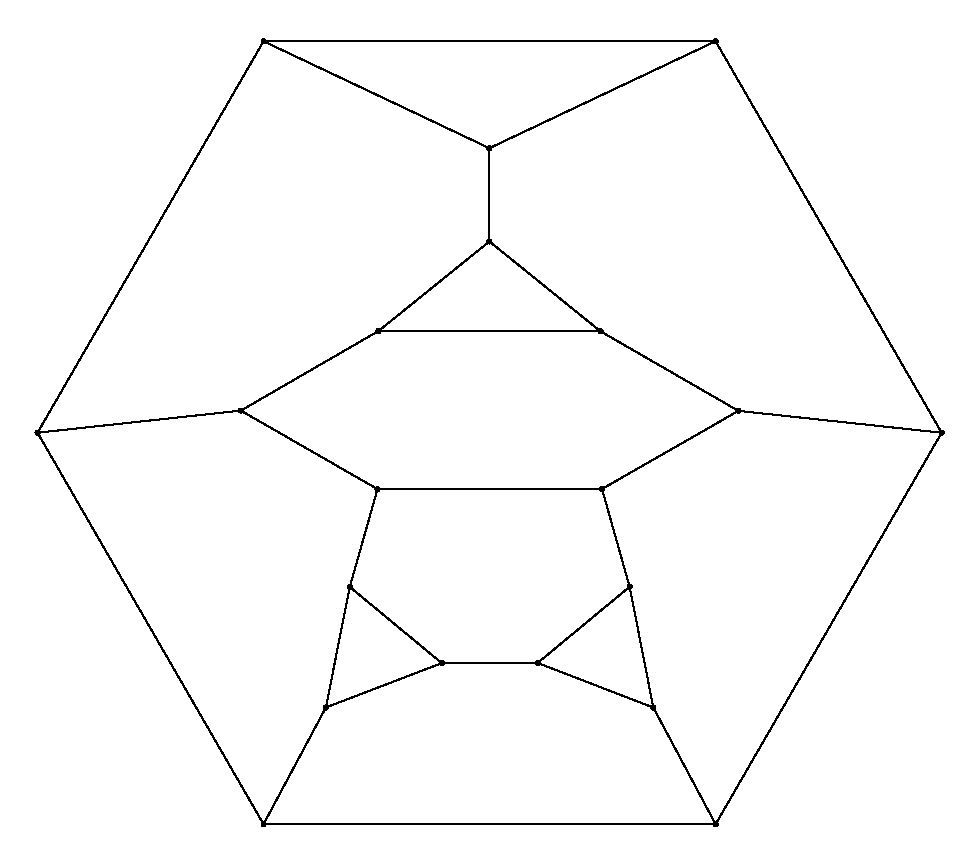
\includegraphics{GOLDBERGpicture/FromTrig.ps}}\par
\end{minipage}
\begin{minipage}{5cm}
\hspace{-1cm}The graph $3_{20}(D_{2d})$
\end{minipage}
\end{center}

\end{slide}






\begin{slide}{$z$- and railroad-structure of graphs $3_n$}

All zigzags and railroads are simple. 
%Denote by $(Z_{i,k})_{1\leq i\leq 3, 1\leq k\leq m_i}$ the zigzags of $G$.

\begin{itemize}
\item The $z$-vector is of the form 
\begin{equation*}
\textcolor{red}{(4s_1)^{m_1}, (4s_2)^{m_2},(4s_3)^{m_3}}\mbox{~~~with~~~}\textcolor{red}{s_im_i=\frac{n}{4}};
\end{equation*}
the number of railroads is $m_1+m_2+m_3-3$.

\item $G$ has $\geq 3$ zigzags with equality if and only if it is tight.

\item If $G$ is tight, then $z(G)=n^3$ (so, each zigzag is a Hamiltonian circuit).

%(iv) $G$ is $z$-balanced and $|Z_{i,k}\cap Z_{j,l}|=\left\lbrace\begin{array}{lcl}
%0               &\mbox{~if~}    &i=j,\\
%\frac{n}{2m_im_j}     &\mbox{~if~}    &i\not= j.
%\end{array}\right.$.

\item All $3_n$ are tight if and only if $\frac{n}{4}$ is prime.

\item There exists a tight  $3_n$ if and only if $\frac{n}{4}$ is odd.
\end{itemize}


\end{slide}




\begin{slide}{Conjecture on $4_n(D_3)$, $4$ parameters}
\vspace{-3mm}
\begin{itemize}
\item For tight graphs $4_n$ of symmetry $D_3$, $D_{3d}$ or $D_{3h}$ the $z$-vector is of the form
\begin{center}
$a^k$ with $k\in \{1, 2, 3, 6\}$\\
or $a^k, b^l$ with $k,l\in \{1, 3\}$.
\end{center}

\item A \textcolor{red}{knotted} $4_n$ of such symmetry has symmetry $D_3$.

\item If there is a knotted $4_n$ of symmetry $D_3$, then $\frac{n}{2}$ is the product of at most $2$ primes.

\end{itemize}



\begin{center}
\begin{minipage}{5cm}
\resizebox{3cm}{!}{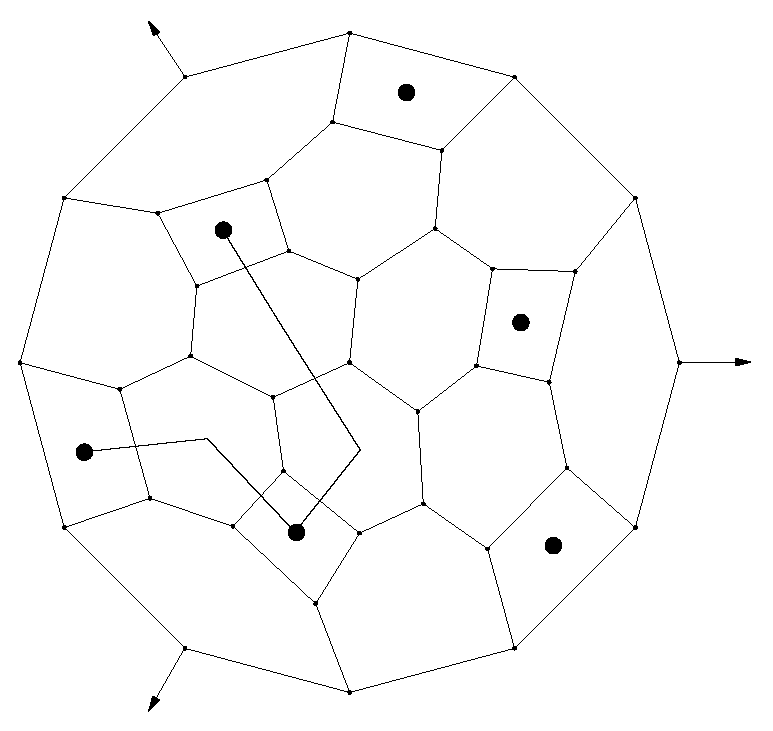
\includegraphics{GOLDBERGpicture/KnotD3_38_4sec.eps}}\par
\end{minipage}
\begin{minipage}{5cm}
First $z$-knotted $4_n$ of symmetry $D_3$.
\end{minipage}
\end{center}

\end{slide}









\begin{slide}{}
\begin{center}
{\Huge 
\begin{tabular*}{6cm}{c}
\\[-0.5cm]
\textcolor{blue}{V. }\textcolor{red}{Zigzags}\\
\textcolor{red}{on}\\
\textcolor{red}{surfaces}
\end{tabular*}
}
\end{center}
\end{slide}


\begin{slide}{Klein and Dyck map}
\begin{center}
\setlength{\unitlength}{1cm}
\begin{minipage}[t]{4.0cm}
\epsfxsize=3.9cm
\epsffile{ZIGZAGpicture/IIIaSec-color.eps}\par
Klein map: $z=8^{21}$
\end{minipage}
\hspace{3cm}
\begin{minipage}[t]{4.0cm}
\epsfxsize=3.9cm
\epsffile{ZIGZAGpicture/IIIbSec-color.eps}\par
Dyck map: $z=6^{16}$
\end{minipage}
\end{center}

\vspace{3mm}

Zigzag, being a local notion, is defined on any surface, even on non-orientable ones.
\end{slide}




\begin{slide}{Regular maps}
A \textcolor{red}{flag-transitive} map is called \textcolor{red}{regular}.

Zigzags of regular maps are simple.
\vspace{3mm}
\begin{center}
\begin{tabular}{||c|c|c|c|l||}
\hline
\hline
map   &$n$  &rot. group       &$z$    &\multicolumn{1}{|c||}{$\QuotS{z(GC_{k,l})}{k^2+kl+l^2}$}\\
\hline
Dod. $\{5^3\}$   &$20$ &$A_5$  &$10^6$         &\textcolor{blue}{$10^6$} or $6^{10}$ or $4^{15}$\\
Klein${}^*$ $\{7^3\}$ &$56$ &$PSL(2,7)$      &$8^{21}$       &\textcolor{blue}{$8^{21}$} or $6^{28}$\\
Dyck${}^*$ $\{8^3\}$  &$32$ &$(*)$   &$6^{16}$       &\textcolor{blue}{$6^{16}$} or $8^{12}$\\
$\{11^3\}$               &$220$&$PSL(2,11)$    &$10^{66}$       &\textcolor{blue}{$10^{66}$} or $6^{110}$ or $12^{55}$\\
\hline
\hline
\end{tabular}
\end{center}
$(*)$ is a solvable group of order $96$ generated by two elements $R$, $S$ subject to the relations $R^3=S^8=(RS)^2=(S^2R^{-1})^3=1$.



\end{slide}




\begin{slide}{Folding a surface}
Let $G$ be a map on a surface $S$ and $f$ a fixed-point free involution on $S$;
denote by $\tilde{G}$ the corresponding map on the folded surface $\tilde{S}$.

\begin{itemize}
\item Zigzags of $G$, which are invariant under $f$, are mapped to zigzags of half-length and half-signature in $\tilde{G}$.

\item If $Z_2=f(Z_1)$ with $Z_2\not= Z_1$, then we put compatible orientation on $Z_i$. Then, the $Z_i$ are mapped to a zigzag $\tilde{Z}$ of $\tilde{G}$ with the signature of $Z_1$ plus the half of the intersection between $Z_1$ and $Z_2$.

\end{itemize}

\textcolor{red}{Example}: Petersen graph embedded on the projective plane is a folding of the Dodecahedron by central inversion.


\end{slide}







\begin{slide}{Lins trialities}
\begin{tabular}{||c|c|c|c||}
\hline
$(\textcolor{red}{v},\textcolor{green}{f},\textcolor{blue}{z})\rightarrow $   &our notation          &notation in [1]  &notation in [2]\\
\hline
$(\textcolor{red}{v},\textcolor{green}{f},\textcolor{blue}{z})$               &${\cal M}$            &gem                   &${\cal M}$\\  %0
$(\textcolor{green}{f},\textcolor{red}{v},\textcolor{blue}{z})$               &${\cal M}^*$          &dual gem              &${\cal M}^*$\\  %1
$(\textcolor{blue}{z},\textcolor{green}{f},\textcolor{red}{v})$               &$phial({\cal M})$     &\textcolor{blue}{phial} gem             &$p((p({\cal M}))^*)$\\  %5
$(\textcolor{green}{f},\textcolor{blue}{z},\textcolor{red}{v})$               &$(phial({\cal M}))^*$ &skew-dual gem         &$(p({\cal M}))^*$\\  %4
$(\textcolor{red}{v},\textcolor{blue}{z},\textcolor{green}{f})$               &$skew({\cal M})$      &\textcolor{red}{skew} gem              &$p(M)$\\  %2
$(\textcolor{blue}{z},\textcolor{red}{v},\textcolor{green}{f})$               &$(skew({\cal M}))^*$  &skew-phial gem        &$p({\cal M}^*)$\\\hline  %3
\end{tabular}
Jones, Thornton (1987): those are only ``good'' dualities.
%ere are no other "good" dualities.

{\scriptsize
\begin{enumerate}
\item S. Lins, {\em Graph-Encoded Maps}, J. Combinatorial

Theory Ser. B {\bf 32} (1982) 171--181.

\item K. Anderson and D.B. Surowski, {\em Coxeter-Petrie Complexes}

{\em of Regular Maps}, European J. of Combinatorics {\bf 23-8} (2002) 861--880.
\end{enumerate}
}


\end{slide}



\begin{slide}{Example: Tetrahedron}
\begin{center}
\begin{minipage}{50mm}
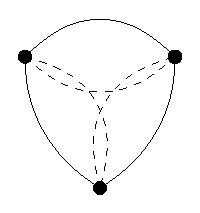
\epsfig{file=ZIG3picture/PhialTetr.eps, height=3cm}\par
$\textcolor{blue}{phial}(Tetrahedron)$
\end{minipage}
\begin{minipage}{50mm}
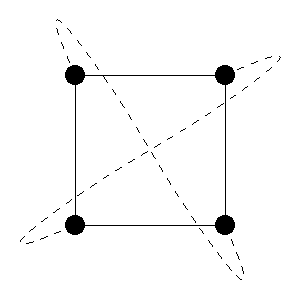
\epsfig{file=ZIG3picture/SkewTetr.eps, height=3cm}\par
$\textcolor{red}{skew}(Tetrahedron)$
\end{minipage}
\end{center}
\begin{center}
two Lins maps on projective plane.
\end{center}

\end{slide}





\begin{slide}{Bipartite skeleton case}

\begin{center}
\begin{minipage}{50mm}
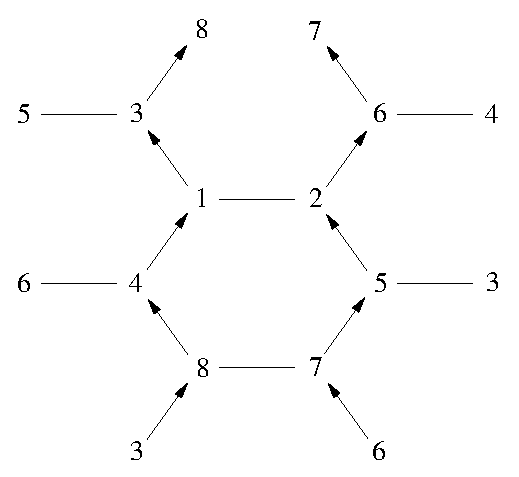
\epsfig{file=ZIG3picture/SkewCube.eps, height=3cm}
\end{minipage}
\begin{minipage}{50mm}
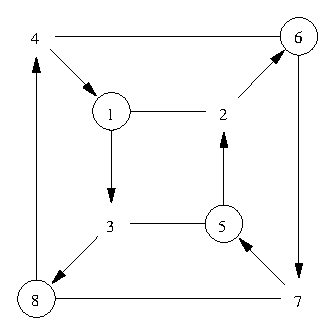
\epsfig{file=ZIG3picture/SkewCubeBip.eps, height=3cm}
\end{minipage}
\end{center}
\begin{center}
Two representation of $\textcolor{red}{skew}(Cube)$: on Torus and as a Cube with cyclic orientation of vertices (marked by 
\epsfig{file=ZIGZAGpicture/Circle.eps, height=4mm}) reversed.
\end{center}
\hspace{0.7cm}
{\it 

{\bf Theorem}

For bipartite graph embedded in oriented surface, the skew operation is, in fact, reversing orientation of one of the part of the bipartition.

}




\end{slide}





\begin{slide}{Prisms and antiprisms}

Let $\chi$ denotes the Euler characteristic.

We conjecture:


\begin{itemize}
\item 
$\textcolor{red}{skew}(Prism_m)$ has $\chi=gcd(m,4)-m$ and is oriented\\
iff $m$ is even;

\item $\textcolor{blue}{phial}(Prism_m)$ has $\chi=2+gcd(m,4)-2m$ and is non-oriented.

\vspace{3mm}

\item $\textcolor{red}{skew}(APrism_m)$ has $\chi=1+gcd(m,3)-2m$ and is non-oriented;


\item $\textcolor{blue}{phial}(APrism_m)$ has $\chi=3+gcd(m,3)-2m$ and is oriented.
\end{itemize}


\end{slide}




\begin{slide}{}
\begin{center}
{\Huge 
\begin{tabular*}{8cm}{c}
\\[-0.5cm]
\textcolor{blue}{VI. }\textcolor{red}{Zigzags}\\
\textcolor{red}{on $n$-dimensional}\\
\textcolor{red}{complexes}
\end{tabular*}
}
\end{center}
\end{slide}



\begin{slide}{Zigzags on $n$-dimensional polytopes}

A \textcolor{red}{flag} $u=(f_0, \dots, f_{n-1})$ is a sequence of faces $f_i$ (of polytope $P$) of dimension $i$ with $f_i\subset f_{i+1}$.

Given a flag $u$, there exist an unique flag $\sigma_i(u)$, which differs from $u$ only in position $i$.

\vspace{3mm}

A \textcolor{red}{zigzag} $z$ is a circuit of flags $(u_j)_{1\leq j\leq l}$, such that $u_j=\sigma_n\dots\sigma_1(u_{j-1})$; the number of flags is called its \textcolor{red}{length}.

\vspace{3mm}

The zigzags partition the flag-set of $P$.

\textcolor{red}{$z$-vector} of $P$ is a vector, listing zigzags with their lengths.

\vspace{3mm}


{\em {\bf Proposition}

If the dimension of polytope is odd, then the length of any zigzag is even.
}

\end{slide}







\begin{slide}{Zigzag of reg. and semireg. \textcolor{red}{$d$-polytopes}}

\vspace{-4mm}
\begin{center}
{\scriptsize
\begin{tabular}{||c|c|c||}
\hline
$d$ &$d$-polytope                        & $z$-vector\\
\hline
$3$&Dodecahedron               &$10^6$\\
%Great Dodecahedron=$\{5,\frac{5}{2}\}$   &                   &\\
%Great Icosahedron=$\{3,\frac{5}{2}\}$   &                   &\\
$4$&$24$-cell                      &$12^{48}$\\
$4$&$600$-cell                     &$30^{240}$\\
$d$&$d$-simplex=$\alpha_d$         &$(n+1)^{n!/2}$\\
$d$&$d$-cross-polytope=$\beta_d$          &$(2n)^{2^{n-2}(n-1)!}$\\
\hline
$4$&octicosahedric polytope            &$45^{480}$\\
$4$&snub $24$-cell                 &$20^{144}$\\
$4$&$0_{21}$=Med($\alpha_4$)       &$15^{12}$\\
$5$&$1_{21}$=Half-$5$-Cube              &$12^{240}$\\
$6$&$2_{21}$=Schl\"afli polytope (in $E_6$)  &$18^{4320}$\\
$7$&$3_{21}$=Gosset polytope (in $E_7$) &$90^{48384}$\\
$8$&$4_{21}$ ($240$ roots of $E_8$)&$36^{29030400}$\\
\hline
\hline
\end{tabular}
}
\end{center}


\end{slide}





\begin{slide}{Reg.-faced and Conway's polytopes}


\begin{center}
{\scriptsize
\begin{tabular}{||c|c|c||}
\hline
$d$&$d$-polytope                        & $z$-vector\\
\hline
$4$&$Pyr(Icosahedron)$             &$25^{12}$\\
$4$&$BPyr(Icosahedron)$            &$40^{12}$\\
$4$&$0_{21}+Pyr(\beta_3)$          &$42^6$\\
$d$&$Pyr(\beta_{d-1})$, $d\geq 4$  &$(\frac{2(d^2-1)}{gcd(d,2)})^{x}$\\
$d$&$BPyr(\alpha_{d-1})$, $d\geq 5$&$(\frac{2d^2}{gcd(d,2)})^{y}$\\
\hline
$4$&Grand Antiprism                &$30^{20}, 50^{40}, 90^{20}$\\
$4$&$C_p\times C_q$                &$(\frac{2pq}{t})^{2t}, (\frac{4pq}{t})^{2t}$\\
&(put $t=gcd(p,q)$)                &if both, $p$ and $q$, are odd\\
&                                   &$(\frac{2pq}{t})^{6t}$, otherwise\\
\hline
\hline
\end{tabular}
}
\end{center}


\end{slide}




\end{document}
